\section{QT Modulation}

Modulation is the reverse of demodulation.
It inputs a stream of (magnitude, angle) vectors and outputs a stream of real
samples. The downsample and upsample processes of modulation are the reverse
of demodulaton's upsample and downsample processes respectively.

\begin{figure}
	\centering
	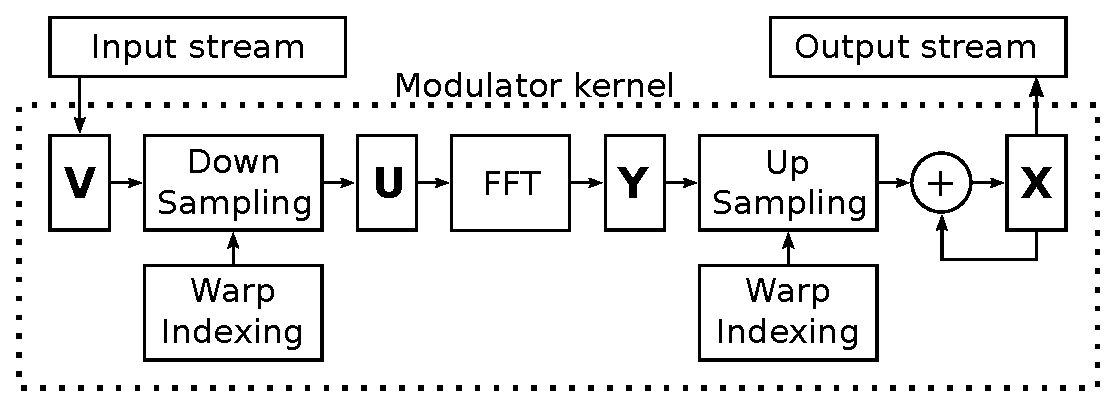
\includegraphics[width=0.95\linewidth]{../source/mod_e}
	\caption[Relative to Quantum Time Demodulation]{Modulation data flow}
	\label{fig:mod}
\end{figure}

%%%%%%%%%%%%%%%%%%%%%%%%%%%%%%%%%%%%%%%%%%%%%%%%%%%%%%%%%%%%%%%%%%%%%%%%%%%%%%%%
\subsection{Downsampling}

V is downsampled to form frequency-domain signal U.
Eq. \ref{eq:eps_j} relates integer index $j$ to fractional index $\epsilon(j)$.
Each point of V can be interpolated into a variable number of U points in a way
that accumulates V points and spits out U points as needed.

Another view is easier to describe mathematically, but needs a logarithm. Let
$\epsilon$ and j be the respective indices of U and V where $\epsilon/j < 1$.
$\epsilon$ is an integer that steps downward from $\epsilon_0$.
\begin{equation}
\epsilon_0 = \frac{N}{2} - 1
\end{equation}

Rewriting equation \ref{eq:eps_j} for $j(\epsilon)$,

\begin{equation}  \label{eq:j_eps}
j(\epsilon) = \left(\frac{N}{2}-1\right)
ln\left(\frac{\epsilon_0}{\epsilon}\right)
\end{equation}

The minimum $\epsilon$ is determined by the span of j.
Let j range from 0 to $v-1$ and $v = 0.469N$.

\begin{equation}
\epsilon(v-1) = \epsilon_0 e^\frac{-(v-1)}{0.5N - 1}
\end{equation}

\begin{equation}
\epsilon(0.469N) = \epsilon_0 e^\frac{-(0.469N-1)}{0.5N - 1}
\approx 0.391 \epsilon_0
\end{equation}

Since $\epsilon$ is always positive, the upchirp case of $R>0$ needs to have its
j index mirrored by using V[v-j], where v is the maximum j such as 0.469N.

%%%%%%%%%%%%%%%%%%%%%%%%%%%%%%%%%%%%%%%%%%%%%%%%%%%%%%%%%%%%%%%%%%%%%%%%%%%%%%%
\subsection{IFFT}

The IFFT ($U \rightarrow Y$) is an Inverse Fast Fourier Transform that
translates N/2 complex frequency values to N/2 complex points in the relative
time domain. These may be assumed to have Hermitian symmetry,
so the imaginary part of $Y$ can be ignored.
It's also possible to realize Y as N real points.

A Hann window is applied to Y after the FFT. Y is then warped and accumulated
in X in a manner similar to the demodulator's correlation function.

%%%%%%%%%%%%%%%%%%%%%%%%%%%%%%%%%%%%%%%%%%%%%%%%%%%%%%%%%%%%%%%%%%%%%%%%%%%%%%%%
\subsection{Upsampling}

The upsampling process of Fig.~\ref{fig:mod} translates the sample pitch of
Y to the sample pitch of X using the reverse of the downsampling process.

Fig.~\ref{fig:upsam} illustrates an interpolation scheme for recreating X from Y.
The slope calculation requires a $1/\lambda$ scale factor.
The expense of division can be avoided by using another instance of exponential
sweep such as that described by Eq. \ref{eq:lambdaApprox}.

The X points are the trapezoidal area under the curve in Fig.~\ref{fig:upsam}.
The \textit{Head} and \textit{Middle} regions produce output points.
The \textit{Tail} result is carried into the next \textit{Head}.

\begin{figure}
	\centering
	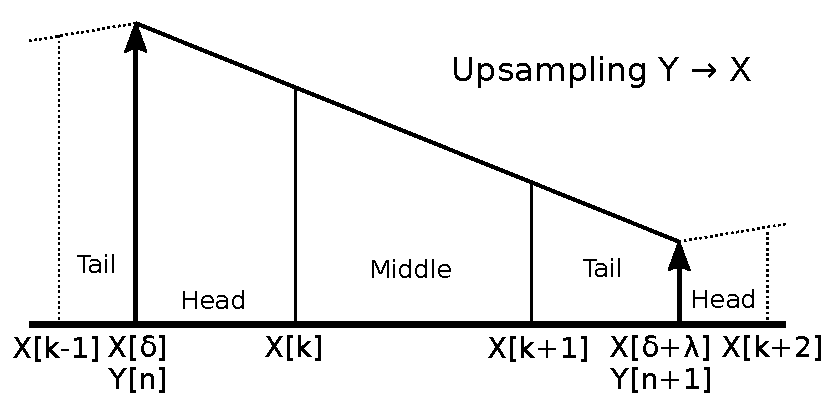
\includegraphics[width=0.8\linewidth]{../source/upsam_e}
	\caption[X interpolation]{Interpolation of Y for upsampling}
	\label{fig:upsam}
\end{figure}

Summation in X is similar to the data flow of Fig.~\ref{fig:wbuf},
but a little easier since X and Y are real (rather than complex) numbers.
X memory is wider than with demodulation to handle accumulation in memory.
